\documentclass[a4paper, 11pt]{article}
\usepackage{comment} 
\usepackage{fullpage} 
\usepackage[spanish]{babel} 
\selectlanguage{spanish}
\usepackage[utf8]{inputenc}
\usepackage{float} 
\usepackage{graphicx}
\usepackage{ marvosym }
\usepackage{amsthm}
\usepackage{amsmath}
\usepackage[sort&compress, numbers]{natbib}
\usepackage{amssymb}
\usepackage{hyperref}
\hypersetup{colorlinks=True, citecolor=blue}
\usepackage{wrapfig}

\begin{document}
\begin{center}
\LARGE \bf Pr\'actica 2\\ Autómata celular
\end{center}

\vspace{1cm} 
\noindent\textbf {Edson Edgardo Samaniego Pantoja} \hfill \textbf{Materia:} Simulación computacional 
\hfill \\
\textbf{Fecha} \today  
\vspace{1cm} 

\section{Introducción}
Esta segunda práctica llamada autómatas celulares es basada en el juego de la vida el cual se representará en dos dimensiones. El estado del autómata se representa con una matriz bidimensional de ceros y unos donde uno es vivo y cero representa muerto. La supervivencia de cada celda revisada por paso será determinada por sus ocho vecinos que lo rodean y en el caso de las orillas y esquinas son menos vecinos.
La regla de supervivencia básica: una celda está viva si exactamente tres vecinos suyos están vivos.

\section{Objetivo}
Diseñar y ejecutar cinco diferentes experimentos en los que se varíe la regla de supervivencia en la vida de la colonia en una malla de 12 por 12 celdas, hasta que mueran todas las celdas o hasta que llegue a su límite fijado de 30 iteraciones, teniendo la misma probabilidad de estar vivo o muerto desde el inicio y graficar los resultados obtenidos para ver el comportamiento por regla.


\section{Simulación}
En esta programación se utiliza como apoyo el código en github de la profesora Elisa Schaeffer \cite{dra}, como inicio es generar la matriz de 12 filas por 12 columnas en las que cada celda tomara un valor, uno o cero con la misma probabilidad de estar vivo o muerto. 
\begin{verbatim}
z=[]
fila = 12
col = 12
matriz = [[randint(0,1) for i in range(fila)]for j in range(col)]
matriz2=[]
matriz3=[]
for x in range(fila):
    for y in range(col):
        print(matriz[x][y],end=' ')
        matriz2.append(matriz[x][y])
        matriz3.append(matriz[x][y])        
    print()
\end{verbatim}
Se crea una variable llamada matriz en la que se especifica que en rango del valor de fila o columna en este caso 12, cada valor cambiara al azar por el comando randint entre cero y uno, para después realizar ciclos for en los que se generara por fila y por columna una matriz donde ya se visualiza los datos aleatorios.
A grandes rasgos una vez teniendo la matriz generada se pasa a analizar celda por celda para saber qué valor es el que está y tomar en cuenta sus ocho o menos vecinos dependiendo la posición para esto como es un código grande se puede consultar en github \cite{Edson}. Las tomas de decisión o reglas del juego de la vida se determinan después de hacer el análisis de la malla inicial y por medio de condiciones if se determina si la suma de vecinos dado en una variable L es menor, mayor o igual a tal valor dado (según la regla) entonces cambiara el valor de la celda central a estado muerto.
\begin{verbatim}
        if pos == 1: # si la celda central está viva 
            if L<=3 : # si la suma de sus vecinos es menor igual a 3
                matriz3[z]= 0 #entonces la celda central cambiara a 0
        if pos == 0:  #condición para crear vida si la celda central es 0 
            if L == 2  :  
                matriz3[z]= 1
\end{verbatim}
Estos ciclos son realizados una cantidad de treinta veces, viéndolo de manera que partiendo de la imagen inicial se crea una máscara que según la regla dada modifica su estado cada celda central respecto a sus vecinos, se genera una nueva matriz a la que se le volverá a aplicar la máscara y así sucesivamente las treinta iteraciones hasta que ya no haya sobrevivientes o si queden unos restantes. Para su visualización paso por paso se genera una figura donde se ven las celdas color negro y blanco según su estado y en forma de matriz 12 por 12.
\begin{verbatim}
    matrix = numpy.matrix(M)   
    fig = plt.figure()
    plt.xlabel('12 columnas')
    plt.ylabel('12 filas')
    plt.imshow(matrix, interpolation='nearest', cmap=plt.cm.Greys)
    fig.suptitle(i + 1)
    plt.savefig('regla1_it1.png')
    plt.show()   
\end{verbatim}
En github \cite{Edson} se puede encontrar los gifs realizados en la página GIPHY \cite{GIPHY}, los gifs hacen que se vea como se fue comportando la matriz conforme se le aplicaba la regla o mascara cada iteración durando en algunos casos hasta las 30 iteraciones para desaparecer o en solo 3 iteraciones mueren las celdas. 
\section{Resultados}

    \begin{table}[H]
        \caption{Resultados de cada regla que se aplico a la matriz donde muestra mínimo y máximo de celdas vivas así como en que paso desapareció}
        \bigskip
        \label{tab1}
        \centering
        \begin{tabular}{|r|rr|r|}
        \hline
        $regla$&$\min$&$\max$&$desapareció$\\
        \hline
        1 & 1 & 42 & 30 \\
        2 & 4 & 31 & 4 \\
        3 & 3 & 40 & 3  \\
        4 & 115 & 142 & No \\
        5 & 2 & 51 & 5\\
        \hline
        \end{tabular}
    \end{table}
   
Para visualizar de manera más detallada cada regla, se realiza una gráfica de barras donde aparece que valor de celdas vivas había en cada iteración que se realizó y se puede ver que cuando llegaba a 0 ya no se podía crear vida por las condiciones dadas.
En esta primer figura \ref{regla1} se aplica una regla 1 de que si la celda central es igual a 1 y si sus vecinos vivos son 3 o menos entonces dicha celda morirá, así como si es una celda muerta y dos de sus vecinos están vivos entonces este cambiara a vivo. Este caso se observó que no lograron sobrevivir las colonias hasta la iteración 30, solo hasta la 29 hubo un número mínimo de 1 celda viva antes de desaparecer.   
\begin{verbatim}
        if pos == 1:  
            if L<=3 : 
                matriz3[z]= 0 
        if pos == 0:  
            if L == 2  :  
                matriz3[z]= 1
                
\end{verbatim}

\begin{figure}[H]
  \centering
  \caption{Gráfica de resultados para la regla 1}  
  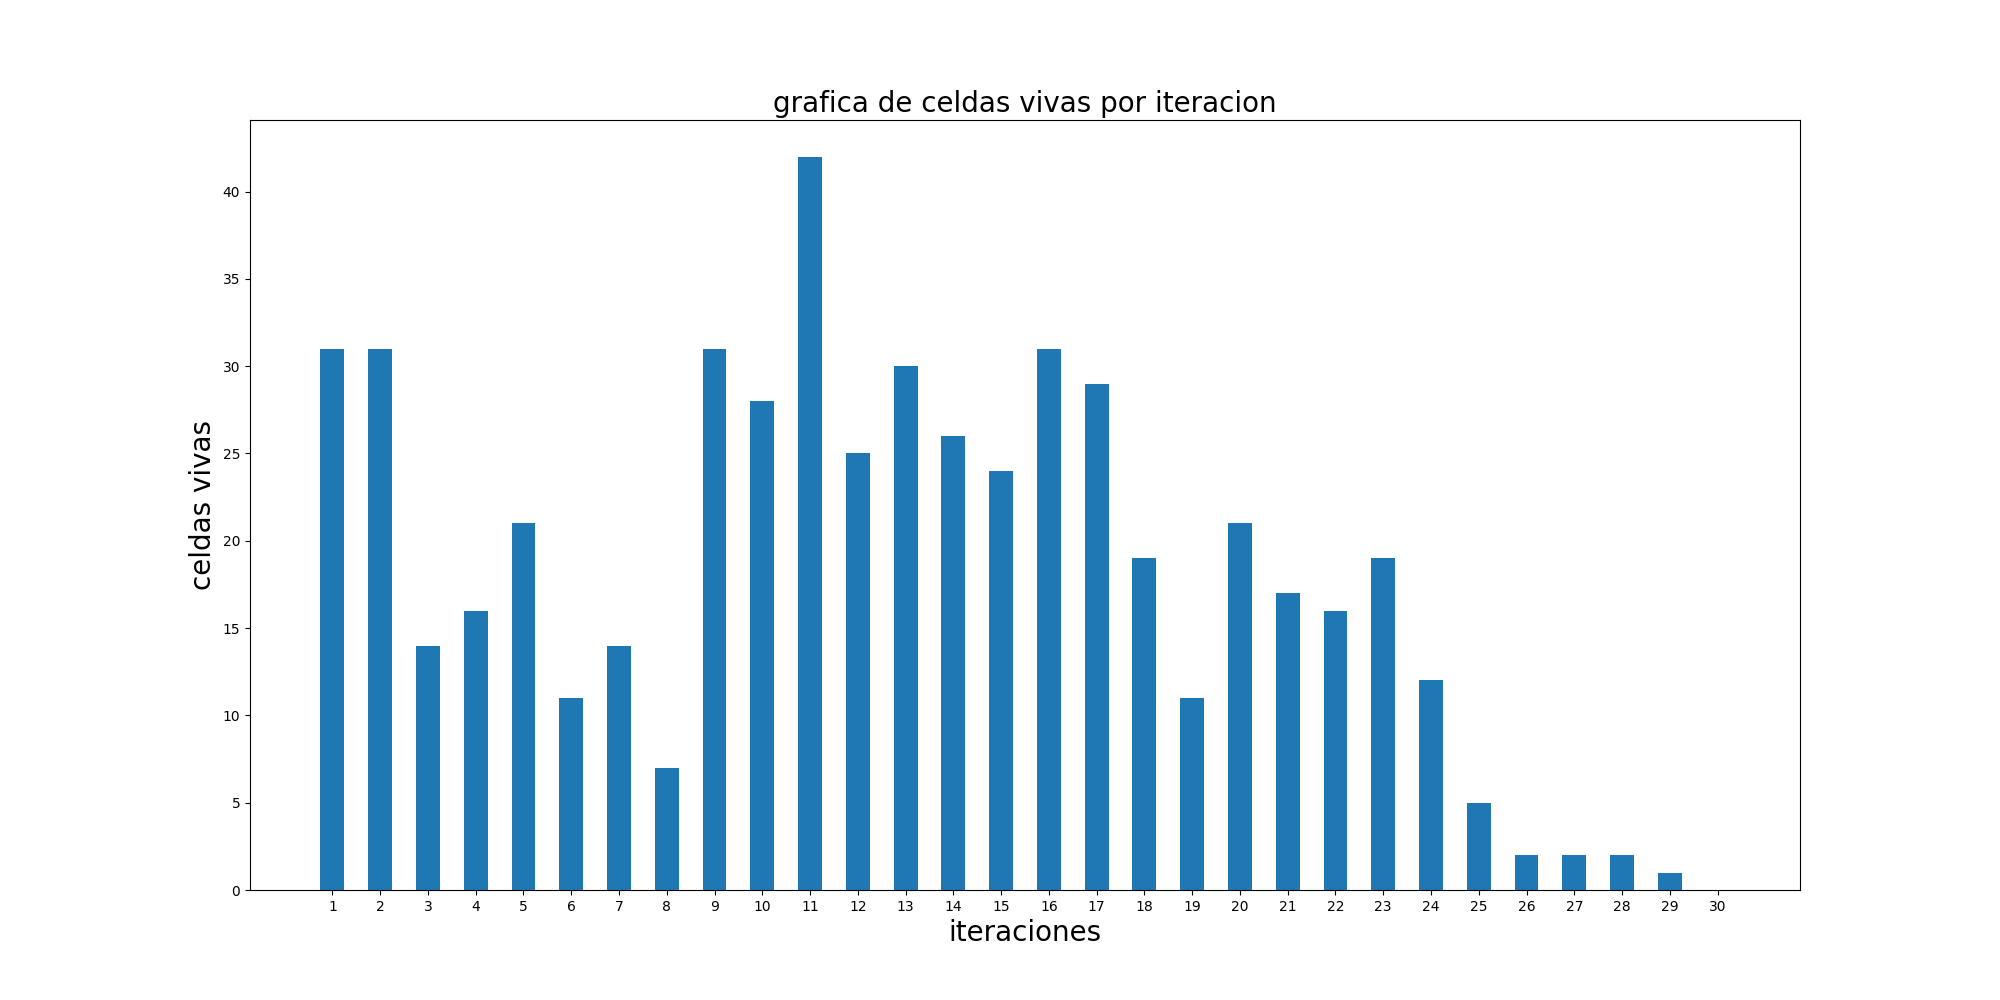
\includegraphics[width=1.2\textwidth]{grafica_regla1.png}
  \label{regla1}
\end{figure}

La segunda regla aplicada se hacen dos condiciones, para el caso en que la celda central este viva y si tres vecinos exactamente están vivos entonces se mantendrá viva la celda pero sí de lo contrario los vecinos no son igual a tres vivos entonces morirá. También se hizo condición para crear vida en caso que la celda sea cero y si tres vecinos son vivos entonces esta celda vivirá.
La figura \ref{regla2} muestra como en solo 4 iteraciones esta colonia desapareció por completo ya que la condición era muy difícil de que se diera, por eso dio saltos grandes al irse reduciendo de manera rápida.
\begin{verbatim}
        if pos == 1:  
            if L==3 : 
                matriz3[z]= 1
            else:
                matriz3[z]= 0
        if pos == 0:  
            if L == 3  :  
                matriz3[z]= 1
\end{verbatim}
\begin{figure}[H]
  \centering      
  \caption{Gráfica de resultados para la regla 2}  
  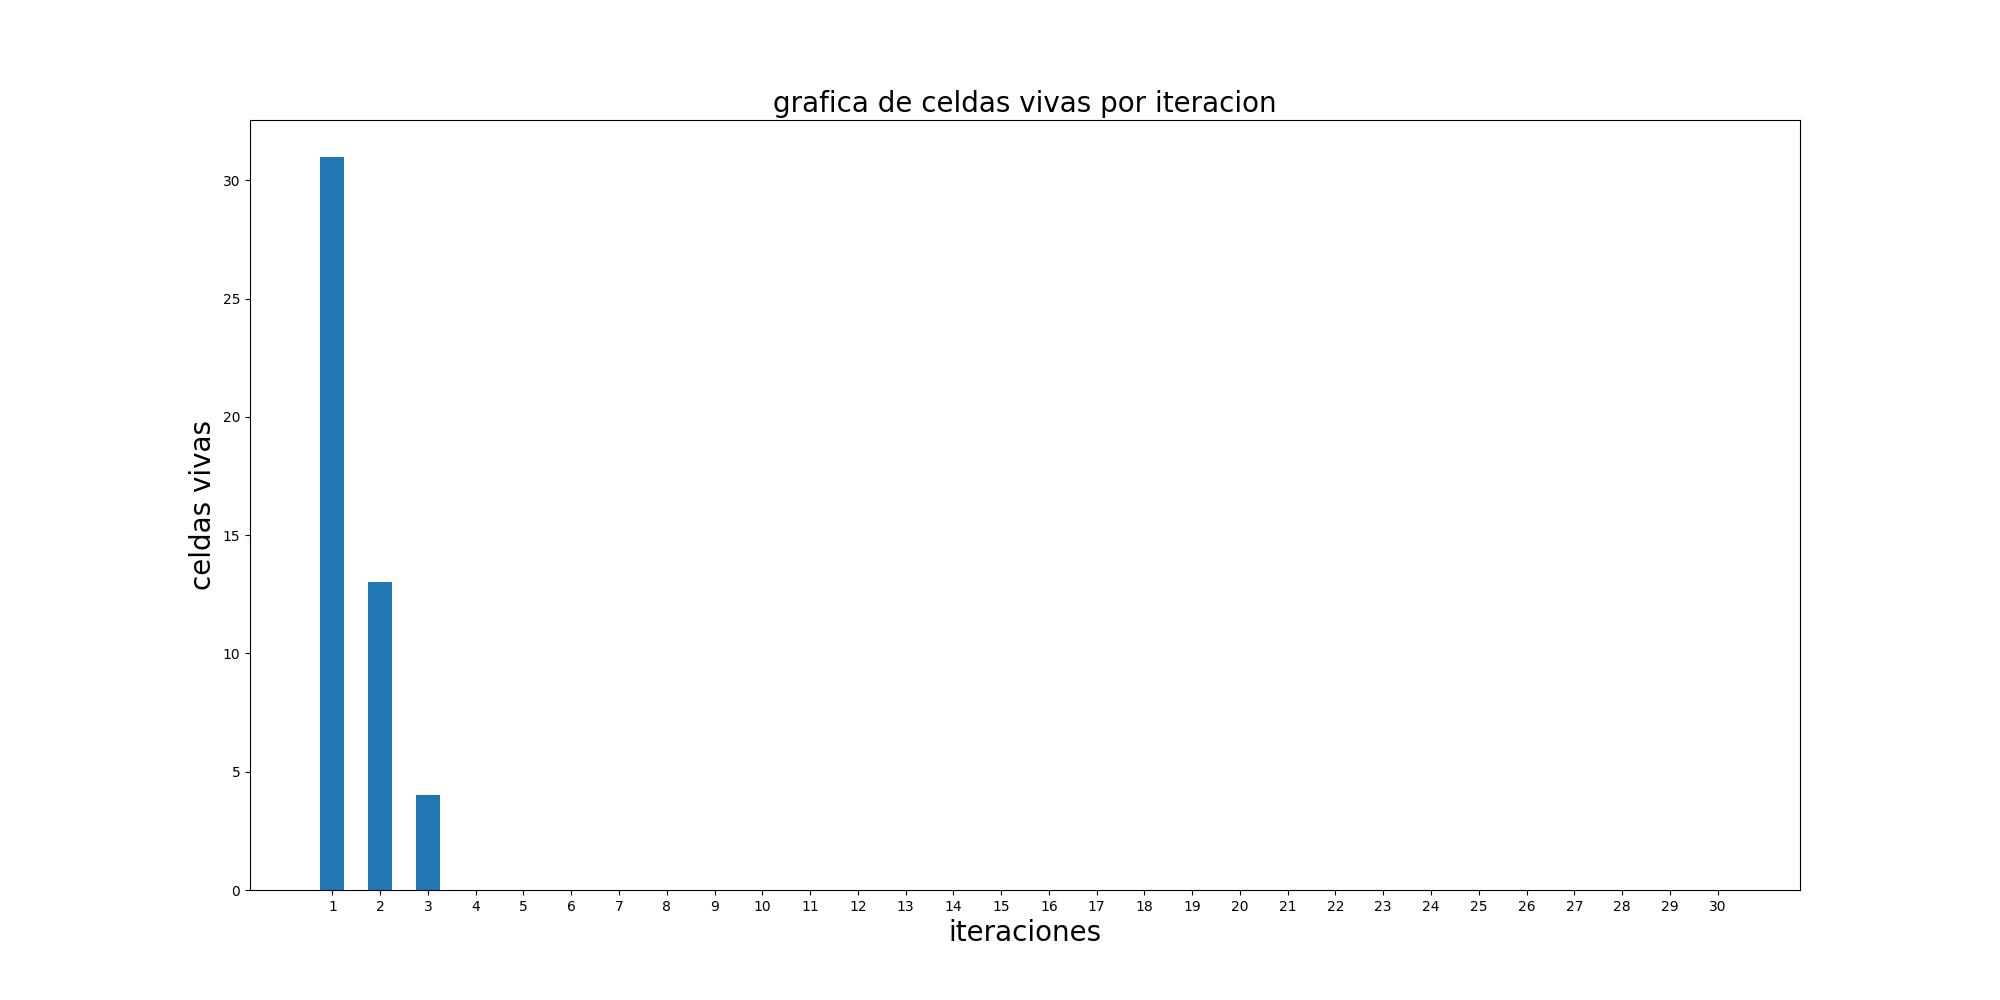
\includegraphics[width=1.2\textwidth]{grafica_regla2.png}
  \label{regla2}
\end{figure}


La tercer regla consistió en una sola condición de supervivencia en que si está vivo el centro y si sus vecinos 4, 5, 6 están vivos entonces este permanecerá vivo y de lo contrario si no son estos morirá la celda. Lo cual para la iteración tres provoco que desapareciera toda la colonia de celdas figura \ref{regla3}.
\begin{verbatim}
        if pos == 1:  
            if 3< L <=6 : 
                matriz3[z]= 1           
            else:
                matriz[z]=0
\end{verbatim}
\begin{figure}[H]
  \centering      
  \caption{Gráfica de resultados para la regla 3}  
  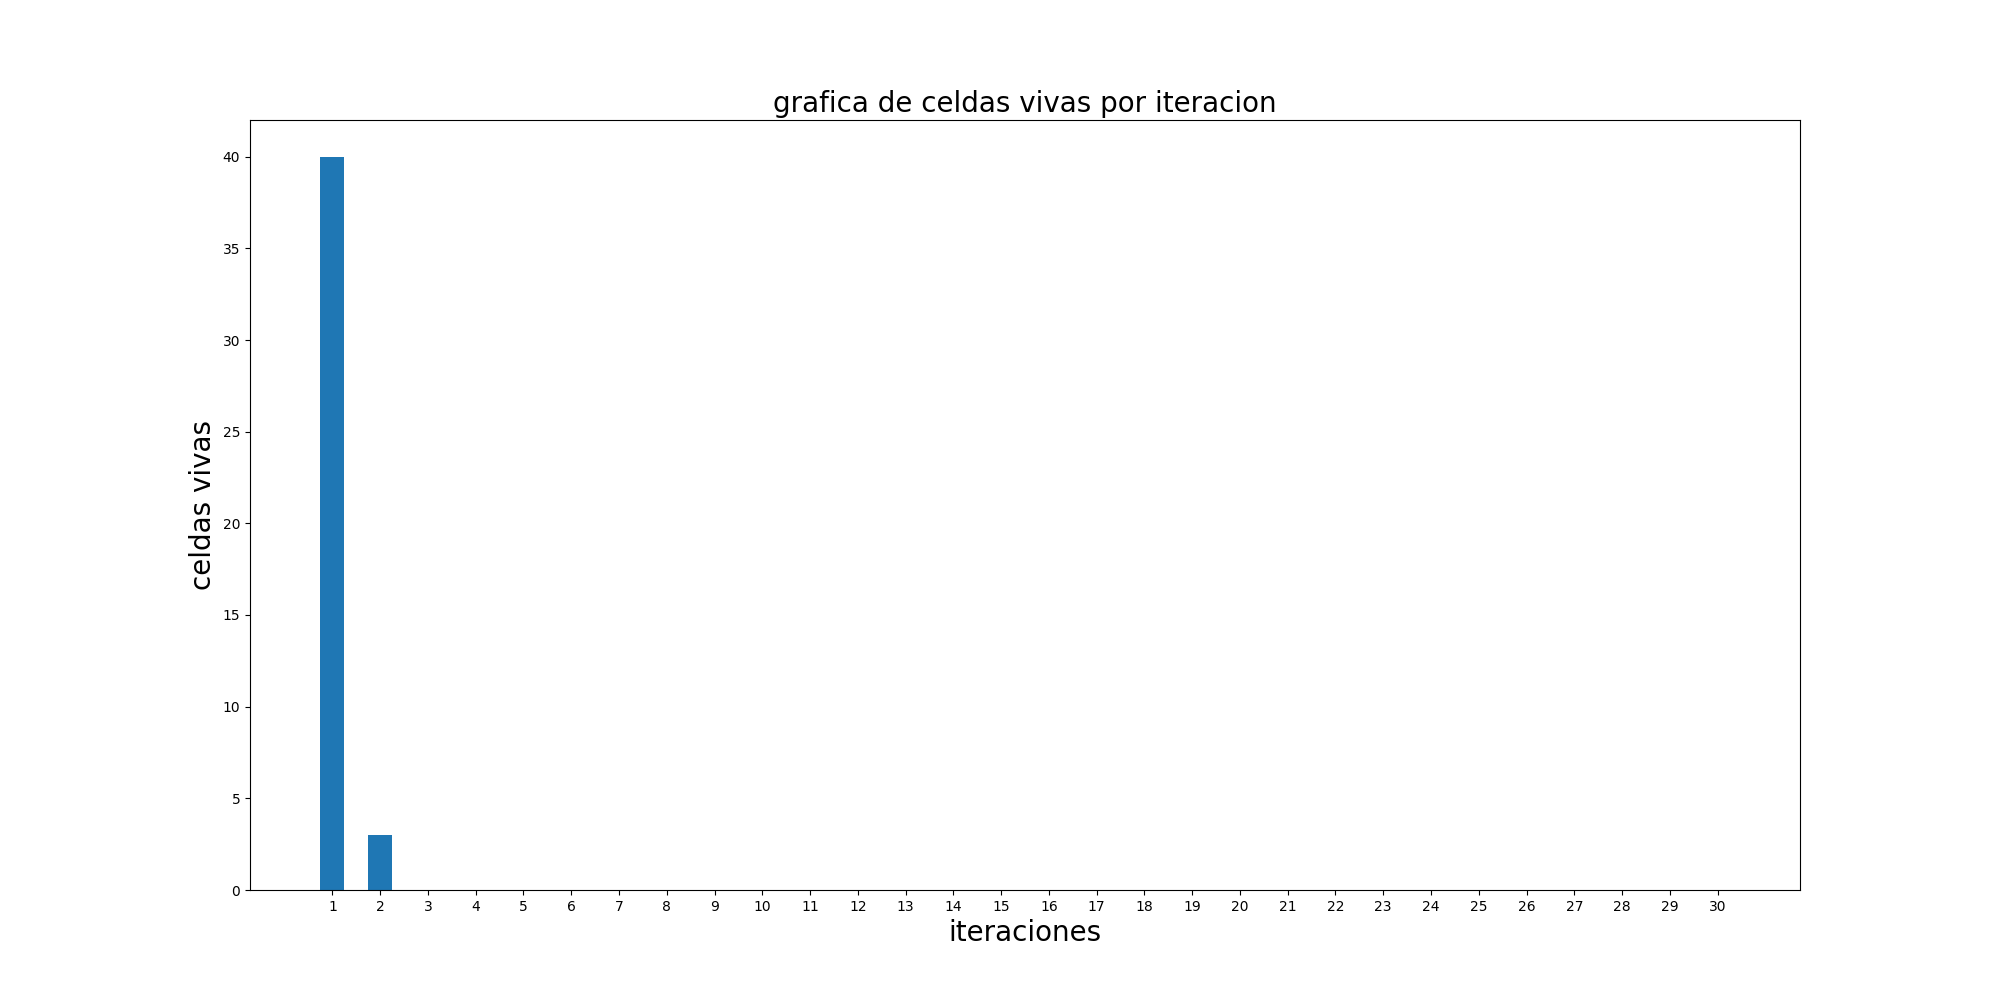
\includegraphics[width=1.2\textwidth]{grafica_regla3.png}
  \label{regla3}
\end{figure}

La regla cuatro fue un caso diferente en su gráfica de barras figura \ref{regla4} ya que se observó que no desapareció a lo largo de 30 iteraciones sino de lo contrario aumento el numero de celdas vivas, esto como consecuencia de experimentar con las condiciones de supervivencia como lo muestra el código siguiente en que si la celda era uno y seis de sus vecinos vivían entonces este moría y caso contrario si la celda era cero y un vecino estaba vivo la celda cambia a uno, esta condición fue la que debería impedir que no murieran tantas celdas. 
\begin{verbatim}
      if pos == 1:  
            if L ==6 : 
                matriz3[z]= 0           
        if pos == 0:
            if L > 2
                 matriz3[z]= 1 
\end{verbatim}
\begin{figure}[H]
  \centering      
  \caption{Gráfica de resultados para la regla 4}  
  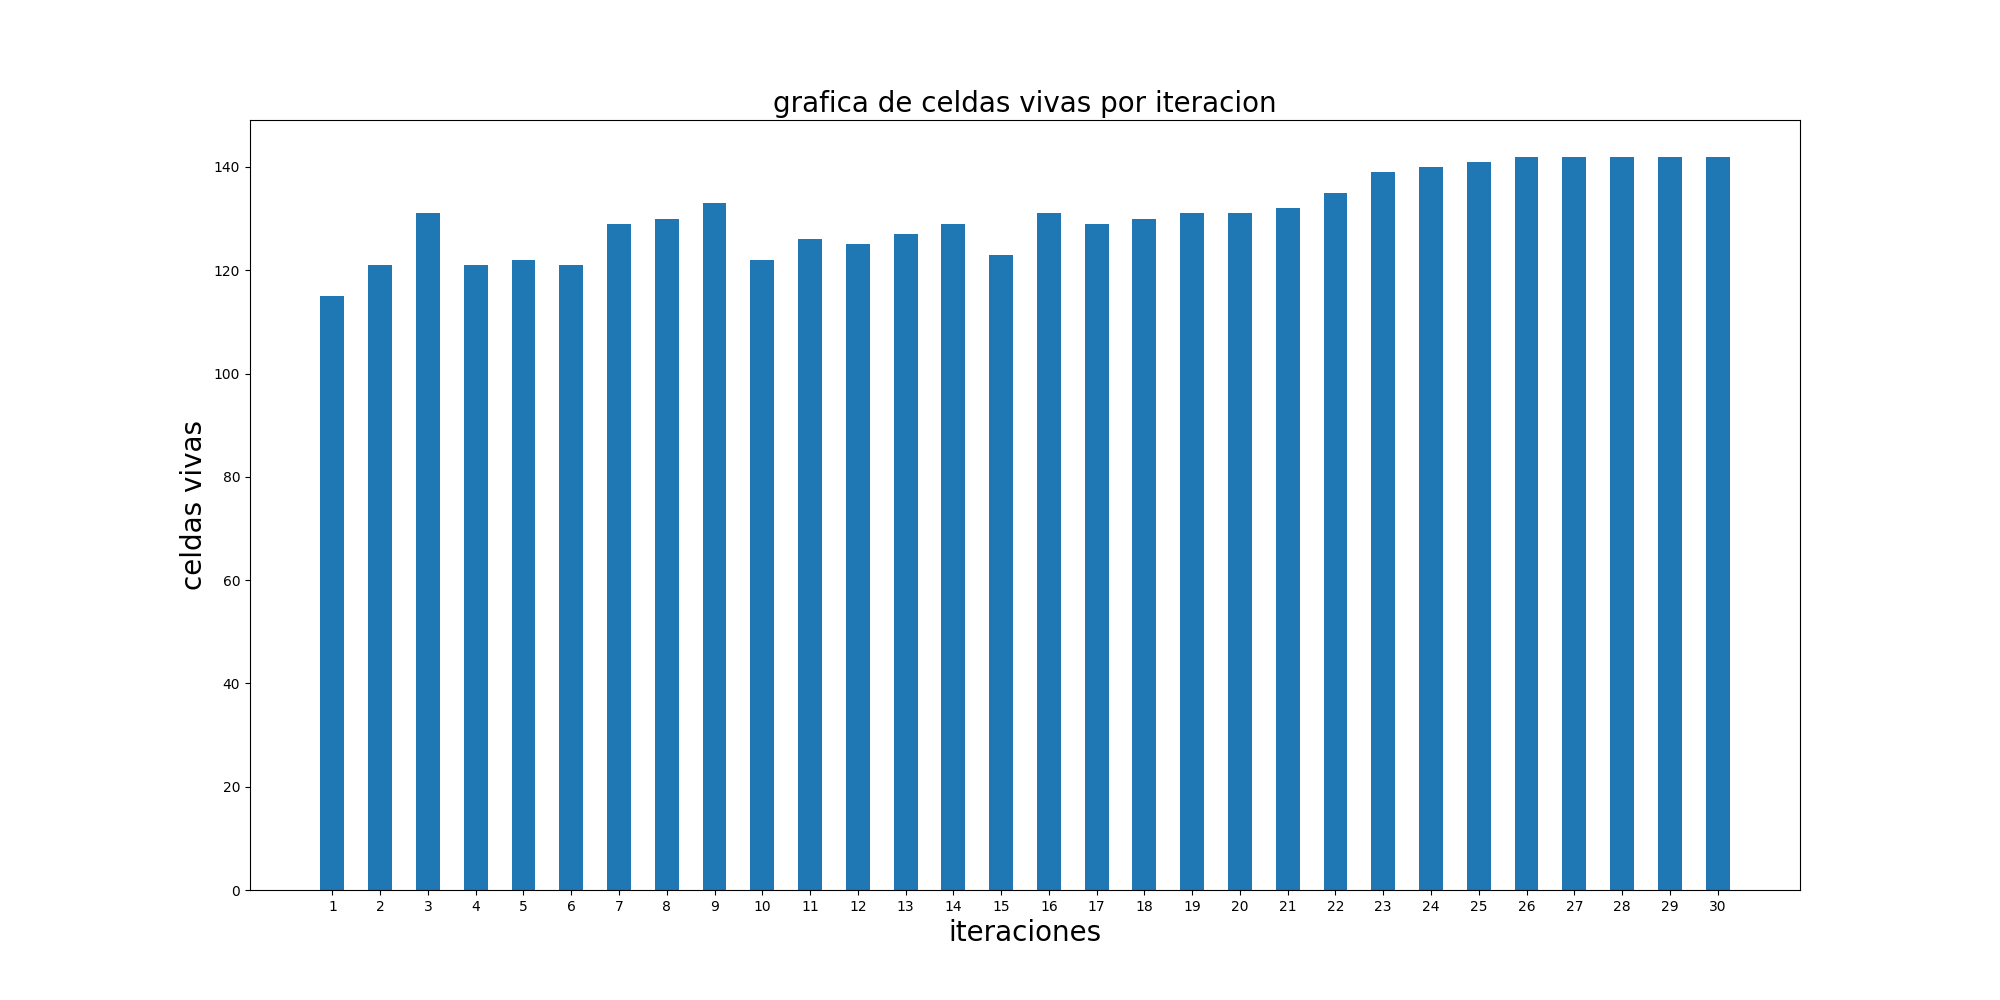
\includegraphics[width=1.2\textwidth]{grafica_regla4.png}
  \label{regla4}
\end{figure}

Ya para la regla cinco se probó el caso en que la celda moriría solo si menos de tres vecinos estaban vivos y caso contrario únicamente si los vecinos cinco y seis estaban vivos. Los resultados se ven en la figura \ref{regla5} donde tuvo una duración hasta la quinta iteración para que desapareciera ya que la condición de vida era muy difícil de coincidir.
\begin{verbatim}
        if pos == 1:  
            if L < 3 : 
                matriz3[z]= 0           
        if pos == 0:
            if 7 > L > 4
                 matriz3[z]= 1 
\end{verbatim}

\begin{figure}[H]
  \centering      
  \caption{Gráfica de resultados para la regla 5}  
  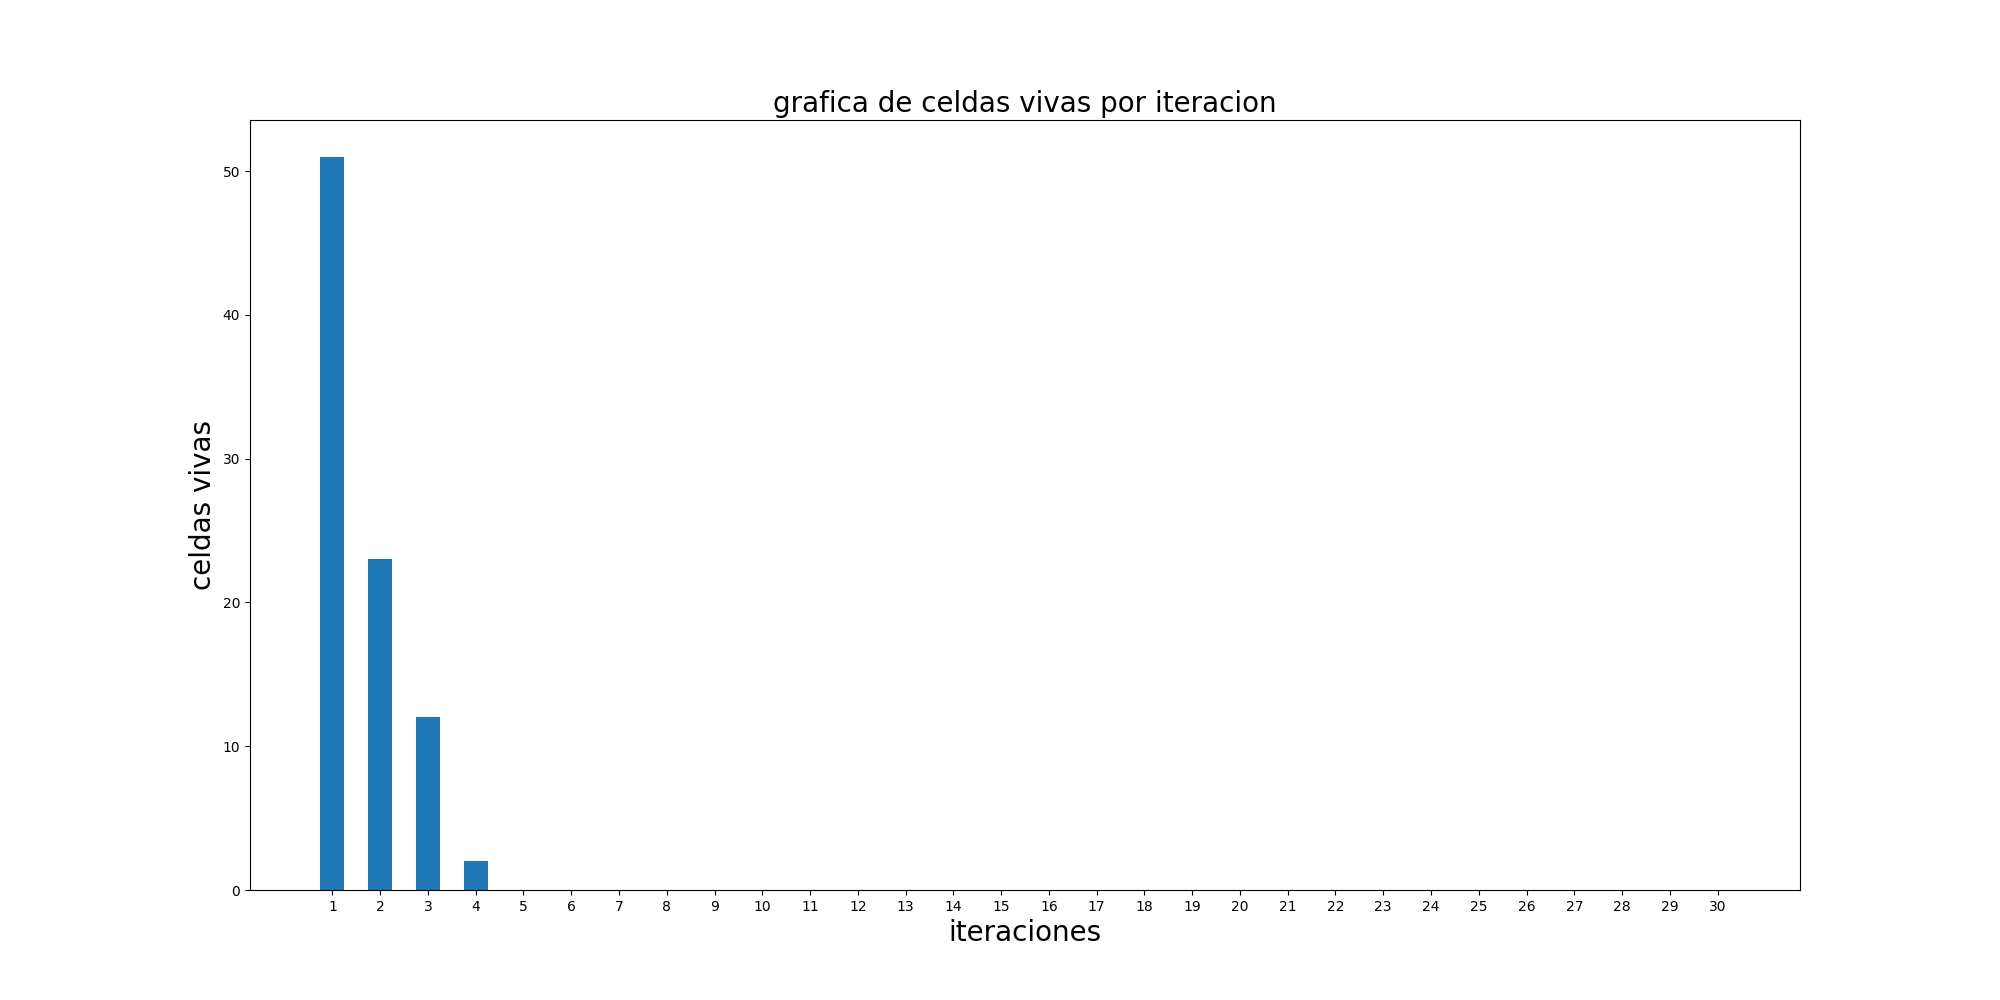
\includegraphics[width=1.2\textwidth]{grafica_regla5.png}
  \label{regla5}
\end{figure}


\bibliography{referencias}
\bibliographystyle{plainnat}




\end{document}
